
Riistvara valikul lähtuti etteantud nõuetest, et loodav juhttorni prototüüp toimiks võimalikult veatult ning töökindlalt. Samuti arvestati ka sellega, et juhttorn oleks võimalikult lihtsasti ümber seadistatav erinevatele laevatüüpidele kasutamiseks. Esitatud nõuded süsteemile olid järgnevad:

\begin{itemize}
\item
  Sisendiks kolm kaamerat, resolutsiooniga vähemalt 1000x1000 pikslit
\item
  Laevade tuvastuskiirus vähemalt 15 kaadrit sekundis
\end{itemize}

Tulevikus plaanitakse taolist süsteemi rakendada erinevatel laevatüüpidel, mistõttu on komponendid valitud laialdaselt kasutatavate ning hõlpsasti saadaolevate seadmete hulgast.

\section{Juhtkontroller ehk pardaarvuti}\label{juhtkontroller-ehk-pardaarvuti}

Juhtkontroller on seade, mis tegeleb selle külge ühendatud kaameratelt saadud informatsiooni töötlemisega ning tulemuste edastamisega autopiloodile. Pardaarvuti asetseb laeva juhttornis, ümbritsetuna kolmest kaamerast. Kaameratelt saadava info peal (antud kontekstis reaalajas video) rakendatakse analüütilisi algoritme, mille väljundina saadakse info (tuvastatud objektid ning nende suhteline asukoht kaadris), mis edastatakse autopiloodile, andes lisainfot ümbritseva keskkonna kohta, mille põhjal viimane teeb otsuse, kuidas laevaga käituda.

Antud ülesande lahendamiseks on saadaval mitmeid monoplaatarvuteid (\emph{Single-Board Computer}, (SBC) \cite{ref19}, \emph{System on Module} (SoM)), populaarseimatena Nvidia Jetson seeria \cite{ref20}, mis on tehisintellekti ning masinnägemise ja masinõppe rakendusteks spetsialiseeritud ja Raspberry Pi \cite{ref21}. Antud ülesande lahendamisel välistame Raspberry Pi valikutest kuna juhttorni süsteem hõlmab 4 kaameraga paralleelselt töötamist, (Raspberry Pi'l ainult 1 kaamerasisend). See vajab rohket arvutusvõimsust, kuid antud seadmel pole selle kohast võimekust, ega vajalikku riistvara (seadme protsessoris on küll integreeritud graafikakaart, kuid antud ülesande lahendamiseks jääb see liiga nõrgaks). Seetõttu paralleelsete toimingute jaoks on eelkõige kasulik eraldiseisev graafikakaart (\emph{Graphics Processing Unit} (GPU) \cite{ref22}) koos spetsialiseeritud graafikatuumadega (\emph{CUDA Cores} \cite{ref23}), mis on Nvidia Jetson arvutite eeliseks.

Jetsonite seeriasse kuuluvad 4 seadet: Nano, TX2, Xavier NX ning AGX Xavier, mille hulgast viimane kõige võimekam (vt Tabel 3.1.1). Nano on kõige algelisem versioon, millega saab lihtsaimaid masinnägemise rakendusi valmistada, TX2 on sellest mõnevõrra võimekam protsessori ning graafikakaardi arvutusvõimsuse kohalt ning Xavier NX ning AGX Xavier on mõeldud tööstuslikkele kasutusaladele ning nende eelisteks on kuue- ja kaheksatuumalised protsessorid ning Volta arhitektuuriga graafikakaardid, mis sisaldavad ka endas maatriksoperatsioonide kiirendeid (\emph{Tensor Cores}) \cite{ref24}, (vt Joonis 3.1.1).

Tabel 3.1.1. Jetson seeria arvutite parameetrid \cite{ref24}

{\def\LTcaptype{none} % do not increment counter
\begin{longtable}[]{@{}
  >{\raggedright\arraybackslash}p{0.2297\linewidth}
  >{\raggedright\arraybackslash}p{0.2297\linewidth}
  >{\raggedright\arraybackslash}p{0.2568\linewidth}
  >{\raggedright\arraybackslash}p{0.2568\linewidth}@{}}
\toprule\noalign{}
\endhead
\bottomrule\noalign{}
\endlastfoot
\textbf{Parameters} & \textbf{Jetson
Nano} & \textbf{Jetson TX2
Series (NX,
TX2i)} & \textbf{Jetson Xavier
Series (NX,
AGX)} \\
AI Performance & 472 GFLOPs & 1.33 TFLOPs & 21/30 TOPs \\
GPU & 128-core
NVIDIA
Maxwell™ & 256-core NVIDIA
Pascal™ & 384/512-core
NVIDIA Volta™
with 48/64
Tensor Cores \\
CPU & Quad-Core Arm
Cortex-A57 & Dual-Core NVIDIA
Denver and
Quad-Core Arm
Cortex-A57 & 6/8-core NVIDIA
Carmel Arm \\
DL Accelerator & \begin{minipage}[t]{\linewidth}\raggedright
\begin{center}\rule{0.5\linewidth}{0.5pt}\end{center}
\end{minipage} & \begin{minipage}[t]{\linewidth}\raggedright
\begin{center}\rule{0.5\linewidth}{0.5pt}\end{center}
\end{minipage} & 2x NVDLA v1 \\
Vision
Accelerator & \begin{minipage}[t]{\linewidth}\raggedright
\begin{center}\rule{0.5\linewidth}{0.5pt}\end{center}
\end{minipage} & \begin{minipage}[t]{\linewidth}\raggedright
\begin{center}\rule{0.5\linewidth}{0.5pt}\end{center}
\end{minipage} & 2x PVA v1 \\
Memory & 4 GB

64-bit LPDDR4 & 4/8 GB

128-bit LPDDR4 & 8/16/32/64 GB

128-bit LPDDR4x \\
Storage & 16 GB & 16/32 GB & 16/35/64 GB \\
CSI Camera & Up to 4
cameras

(up to 18
Gbps) & \begin{minipage}[t]{\linewidth}\raggedright
Up to 5/6
cameras\\
(up to 30 Gbps)\strut
\end{minipage} & Up to 6 cameras

(up to 62 Gbps) \\
\end{longtable}
}

Eeldusel et vaja on analüüsida kolmest kaamerast tulevat infot paralleelselt ning täpselt, oleks kõige mõistlikum kasutada Xavier seeria süsteemi. Seda just seetõttu, et võrreldes teiste seeriatega on Xavier seeria arvutite jõudlus tagatud suurema hulga graafikakaardi tuumadega, uuema arhitektuuriga (Volta \cite{ref25}), mis sisaldab endas maatrikskiirendeid (\emph{Tensor Cores}, mida vajavad närvivõrgud maatriksarvutustes) ning süvaõppe kiirendeid (\emph{Deep Learning Accelerator}), mis võimaldavad mitme kaamera sisendiga tõhusamalt operatsioone teha.

Antud seerias on valikus nii NX kui ka AGX Jetsonid, mille hulgast on valitud parimad kandidaadid (vt Tabel 3.1.2). Nende hulgast sobilikuim on Jetson AGX Xavier, sest antud seade peab olema võimeline jooksutama mahukat närvivõrku ning tegelema mitme operatsiooniga korraga (kaameratelt info lugemine, info töötlemine närvivõrgus, töödeldud info kujutamine väljundvideol), mis nõuab suurt hulka arvutuslikku ressurssi.

Tabel 3.1.2. Jetson AGX Xavieri ja Xavier NXi parameetrid \cite{ref24}

{\def\LTcaptype{none} % do not increment counter
\begin{longtable}[]{@{}
  >{\raggedright\arraybackslash}p{0.1944\linewidth}
  >{\raggedright\arraybackslash}p{0.3241\linewidth}
  >{\raggedright\arraybackslash}p{0.4630\linewidth}@{}}
\toprule\noalign{}
\endhead
\bottomrule\noalign{}
\endlastfoot
\textbf{Parameters} & \textbf{Jetson AGX Xavier} & \textbf{Jetson Xavier NX 16GB} \\
AI Performance & 32 TOPs & 21 TOPs \\
GPU & \begin{minipage}[t]{\linewidth}\raggedright
512-core NVIDIA Volta™ GPU with\\
64 Tensor Cores\strut
\end{minipage} & 384-core NVIDIA Volta™ GPU with 48 Tensor Cores \\
CPU & \begin{minipage}[t]{\linewidth}\raggedright
8-core NVIDIA Carmel Arm®v8.2\\
64-bit CPU\\
8MB L2 + 4MB L3\strut
\end{minipage} & \begin{minipage}[t]{\linewidth}\raggedright
6-core NVIDIA Carmel Arm®v8.2 64-bit CPU\\
6MB L2 + 4MB L3\strut
\end{minipage} \\
DL Accelerator & 2x NVDLA v1 & 2x NVDLA v1 \\
Vision Accelerator & 2x PVA v1 & 2x PVA v1 \\
Memory & \begin{minipage}[t]{\linewidth}\raggedright
32 GB 256-bit LPDDR4x\\
136,5 GB/s\strut
\end{minipage} & \begin{minipage}[t]{\linewidth}\raggedright
16 GB 128-bit LPDDR4x\\
59,7 GB/s\strut
\end{minipage} \\
Storage & 32 GB eMMC 5.1 & 16 GB eMMC 5.1 \\
CSI Camera & Up to 6 cameras (up to 62 Gbps) & Up to 6 cameras (up to 30 Gbps) \\
\end{longtable}
}

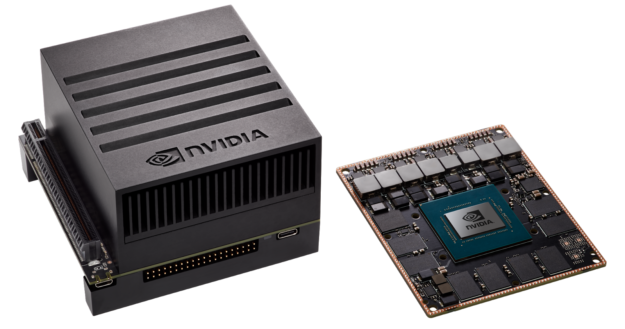
\includegraphics[width=4.09763in,height=2.08472in]{media/image7.png}

Joonis 3.1.1. Valitud arvuti: Jetson AGX Xavier (paremal ilma jahutusplokita) \cite{ref26}

\section{Tensorituumad ja CUDA}\label{tensorituumad-ja-cuda}

Tensorituumade (\emph{Tensor Core'ide}) puhul on tegemist programmeeritavate maatrikstehete kiirenditega, mis viivad läbi operatsioone CUDA \cite{ref23} tuumadega paralleelselt. Antud tuumad rakendavad uuemat sorti ujukomaarvudega ja täisarvudega teostatavad tehted HMMA (\emph{Half-Precision Matrix Multiply and Accumulate}) ja IMMA (\emph{Integer Matrix Multiply and Accumulate}), mille mõjul lineaarsed tehted, signaalitöötlus ning süvaõppeinterferents kiirenevad \cite{ref27} (vt Joonis 3.2.1).

\begin{figure}
\centering
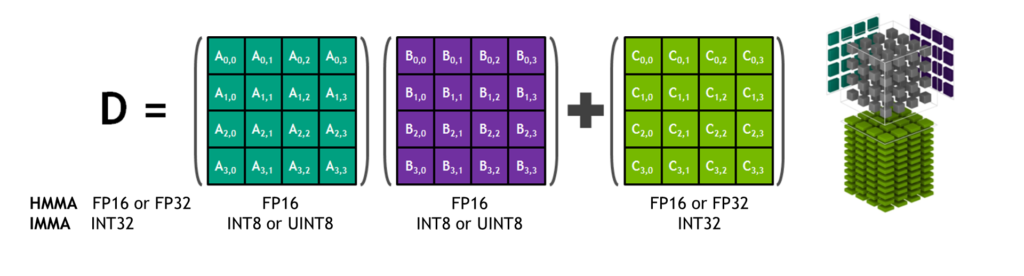
\includegraphics[width=6.10278in,height=1.64514in,alt={Jetson Xavier Tensor Core Matrix diagram}]{media/image8.png}
\caption{Jetson Xavier Tensor Core Matrix diagram}
\end{figure}

Joonis 3.2.1. Tensor Core, kolmedimensiooniliste 4x4x4 maatriksite korrutamine ning summeerimine \cite{ref27}

CUDA puhul on tegemist paralleelarvutuseks mõeldud platvormi ning programmeerimise mudeliga, mis suurendab tehtavate arvutuste hulka mitmekordselt, kasutades selleks protsessori asemel graafikakaarti \cite{ref23}.

CUDA eesmärgiks on kiirendada paralleelarvutusi ning CUDA tuum on analoogne protsessori tuumaga. Ainukeseks erinevuseks on nende ehitus, protsessori tuum on võimeline lahendama kompleksseid arvutusi jadamisi, CUDA tuum lihtsamaid arvutusi graafikakaardis. Eeliseks graafikakaardil protsessori ees on see, et CUDA tuumasid on ühele kiibile paigutatud tuhandeid, mis võimaldab komplekssed arvutused jagada mitmete tuumade vahel ära ning seetõttu ka sooritada arvutused kiiremini, kui protsessor väiksema arvu võimekamate tuumadega. Antud tehnoloogia on integreeritud ning laialdaselt kasutusel masinõppe vallas Nvidia poolt.

\section{Kaamerad}\label{kaamerad}

Kaamerate puhul tuleb arvestada mitmete parameetritega, et tagada süsteemi nõuetekohasus ning edukas toimimine. Kuna antud ülesandes asetseb masinnägemissüsteem juhttornis, mis kinnitub laeva mastile, tuleb kindlasti arvestada sellega et kaamerad või seade kuhu nad asetatakse, peavad võimelised töötama laialdastes temperatuurivahemikes ning muutlikes ilmastikuoludes. Samuti tuleks kaamera tarkvara puhul eelistada üldjuhul värskeimat ja selgelt dokumenteeritud materjali ning arvestada selle ühilduvust juhtarvutiga. See tagab parema kaamera konfigureerimise ning võimaldab ka seeläbi rakendatavat masinnägemistarkvara hõlpsamini hallata.

Kaamerate valikul arvestati järgnevate parameetritega:

\begin{itemize}
\tightlist
\item
  \textbf{Resolutsioon} (pikslites, px) -- otseselt seotud objektide tuvastustäpsusega ning tuvastuskiirusega. Mida väiksema resolutsiooniga sisend antakse tuvastusalgoritmile, seda ebatäpsem/ebakindlam on närvivõrgu ennustustulemus. Sel juhul on tuvastusprotsessi kiirus suurem, kuna algoritm tegeleb väiksema andmehulgaga, millega arvutusprotsesse on vähe, mis lõpptulemusena parandab interferentsi kiirust.
\end{itemize}

\begin{quote}
Suurema resolutsiooni korral paraneb seega tuvastustäpsus kuid väheneb interferentsi kiirus, sest sisendandmete hulk suureneb. Suure resolutsiooniga fotol on rohkem informatsiooni, mis omakorda võimaldab närvivõrgul kindlamaid ennustusi anda.
\end{quote}

\begin{itemize}
\item
  \textbf{Kaadrisagedus} (\emph{Frames per second} -- kaadrit sekundis, FPS) -- parameeter, mis kirjeldab kaamera informatsioonivoo edastuskiirust ehk suhet edastatava kaadrihulga ning aja vahel. Suur kaadrisagedus tagab visuaalselt sujuvama andmevoo kuvamise ning lihtsama jälgitavuse, samuti on ka andmekadu väiksem. Väikese kaadrisageduse korral oleks objekti jälgimine ning teekonna ennustamine oluliselt raskem, sest visuaalselt on objekti liikumine katkendlik ning seetõttu ka närvivõrgu ennustuste täpsus halvatud.
\item
  \textbf{Värvussensor} (mono-, polükromaatiline sensor) -- ehk ühevärviline või mitmevärviline sensor. Ühevärviline sensor on sobilik keskkondadesse, kus objekti ning keskkonna vaheline värvikontrast on suur, tagades efektiivse objektituvastuse. Kuna tegemist on monokromaatilise pildiga, siis iga piksli kohta esitatakse üks väärtus, mis jääb kindlasse vahemikku (üldjuhul 0\ldots255 või 0.0\ldots1.0)
\end{itemize}

\begin{quote}
Polükromaatiline sensor sobib seevastu keskkonda, kus kontrast tausta ja objekti vahel ei ole kuigi suur või objekti tuvastamine nõuab rohkem informatsiooni. Sellisel moel pildi edastamisel esitatakse kolm väärtust maatriksina, RGB (vastavalt Red -- punane, Green -- roheline, Blue - sinine) värvustena vahemikes (0\ldots255 või 0.0\ldots1.0, näiteks {[}255, 0, 255{]}). Taoline edastusviis on andmete hulgalt kolm korda mahukam kui monokromaatilise pildi edastamisel, kuna iga piksli kohta esitatakse kolm väärtust.
\end{quote}

Seadmed, mis eelmainitud parameetrile vastaksid on järgnevad (vt Tabel 3.3.1):

Tabel 3.3.1. Parameetritele sobilikud kaamerad

{\def\LTcaptype{none} % do not increment counter
\begin{longtable}[]{@{}
  >{\raggedright\arraybackslash}p{0.1753\linewidth}
  >{\raggedright\arraybackslash}p{0.2371\linewidth}
  >{\raggedright\arraybackslash}p{0.1856\linewidth}
  >{\raggedright\arraybackslash}p{0.1134\linewidth}
  >{\raggedright\arraybackslash}p{0.1134\linewidth}
  >{\raggedright\arraybackslash}p{0.1340\linewidth}@{}}
\toprule\noalign{}
\endhead
\bottomrule\noalign{}
\endlastfoot
\textbf{Kaamera
nimi} & \textbf{Resolutsioon(px)} & \textbf{Kaadrisagedus
(FPS)} & \multicolumn{2}{>{\raggedright\arraybackslash}p{0.2268\linewidth + 2\tabcolsep}}{%
\textbf{Töötemperatuur
(°C)}} & \textbf{Liides} \\
SurveilsQUAD -
Sony IMX290
System \cite{ref28} & 1920x1080 & 120 & -30 & 85 & CSI \\
OpenCV AI Kit:
OAK---D \cite{ref29} & 1280x800 (stereo)
4056x3040 (keskmine) & 120 (stereo)

60 (keskmine) & N/A & N/A & USB-C/PoE \\
OpenCV AI Kit:
OAK---1-PoE
\cite{ref30} & 4056x3040 & 60 & N/A & N/A & USB-C/PoE \\
Atlas IP67 7.1
MP Model
\cite{ref31} & 3208x2200 & 74 & -20 & 55 & PoE \\
Atlas IP67 2.8
MP Model
\cite{ref32} & 1936x1464 & 173 & -20 & 55 & PoE \\
Arducam 12MP
IMX477 \cite{ref33} & 4056x3040 & 60 & N/A & N/A & USB-C \\
Arducam
Fisheye Camera
\cite{ref34} & 2592×1944 & 30 & N/A & N/A & CSI ja
Ethernet \\
\end{longtable}
}

*N/A -- andmed puuduvad

Töö kirjutamise hetkel kasutati algselt SurveilsQUAD kaameraid, kuna need olid antud arvutisüsteemi jaoks eelnevalt ette valmistatud ning projektis olevate osapoolte poolt olid ka Xavierile vastavad tarkvaralised muudatused tehtud arvutisüsteemide instituudis. Lõputöö kirjutamise käigus valmiv projekt oli arendusfaasis, mistõttu oli ka eelarve piiratud ning piirduti esialgu kaameratega, millel oli katsetuste jaoks põhivõimekus olemas. Juhttorni disaini käigus selgus, et valitud kaamerate paigutus oli lühikeste kaablite tõttu piiratud ning tootja ei tarninud seadmetele pikemaid kaableid.

Seetõttu sai valitud Arducam Mini kaamera (vt Joonis 3.3.1), mis ühendati raspberry pi külge ning omakorda etherneti kaabliga Ethernet switchi ning sealt lõpuks Jetson Xavieri külge. Sellega lahendus ka kaablite pikkuse probleem ning samuti oli võimalik ka Xavierile installeerida värskeim tarkvara, mida eelmiste kaamerate vananenud draiverid ei toetanud.

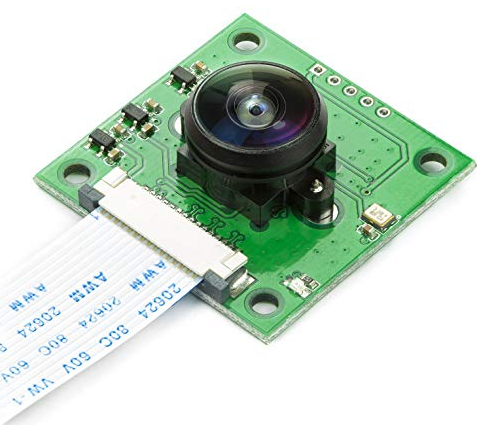
\includegraphics[width=2.75104in,height=2.42839in]{media/image9.png}

Joonis 3.3.1. Arducam Fisheye kaameraga moodul \cite{ref34}

\section{Juhttorn}\label{juhttorn}

Juhttorn asetseb laeva vööris (vt Joonis 3.4.2) ning selle ülesanne on laeva juhtimine üle võtta laeva kapteni käsul ning tegeleda sellega autonoomselt võimalikult vähese kapteni sekkumisega. Selleks on tornil olemas aju Jetson AGXi kujul, mis tegeleb kõikidest anduritest ning kaameratest saadava info kogumise, töötlemise ning seejärel juhtimisotsuse edasi saatmisega autopiloodile, mis omakorda saadab signaalid laeva mootoritele ja tüürile. Jetson saab infot oma ümbritseva keskkonna kohta kaameratest, X-band radarist, AISist ning ilmajaamast tuuleanduri kujul. Andmevahetus juhttorni süsteemis toimub läbi etherneti jaoturi ning 4G ruuteri mis võimaldab saata ning vastu võtta andmeid kasutajalt. Samuti on võimalik arendajatel teha tarkvara uuendusi laeva süsteemidele. AIS (Automaatne Identifitseerimise Süsteem) aitab määrata laeva asukoha teiste meresõidukite suhtes, kasutades satelliite, radar tuvastab punktipilvedega lähedasemaid objekte ning kaamerad ja nendel jooksev masinnägemine tuvastab objektide hulgast laevu ja teisi meresõidukeid. AIS, radar ning kaamerad masinnägemisega täiendavad üksteist, aidates laeval enda ümbruskonda tuvastada ning selles orienteeruda. Süsteemi toidab alalisvooluallikas (vt Joonis 3.4.1). 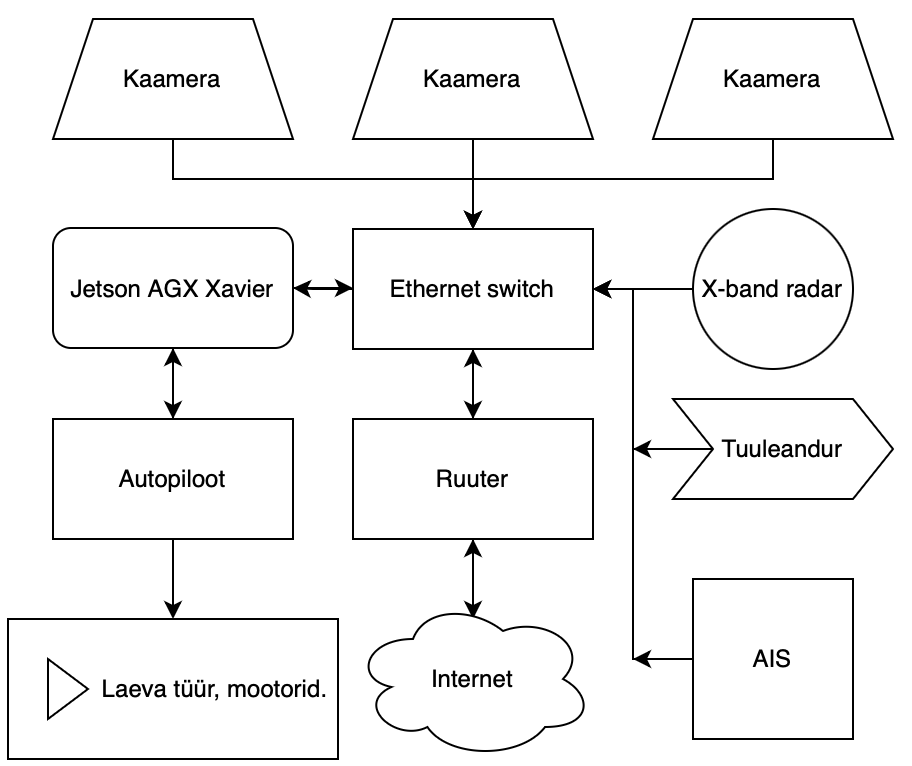
\includegraphics[width=6.10208in,height=5.125in]{media/image10.png}Joonis 3.4.1. Juhttorni lihtsustatud toimimisskeem

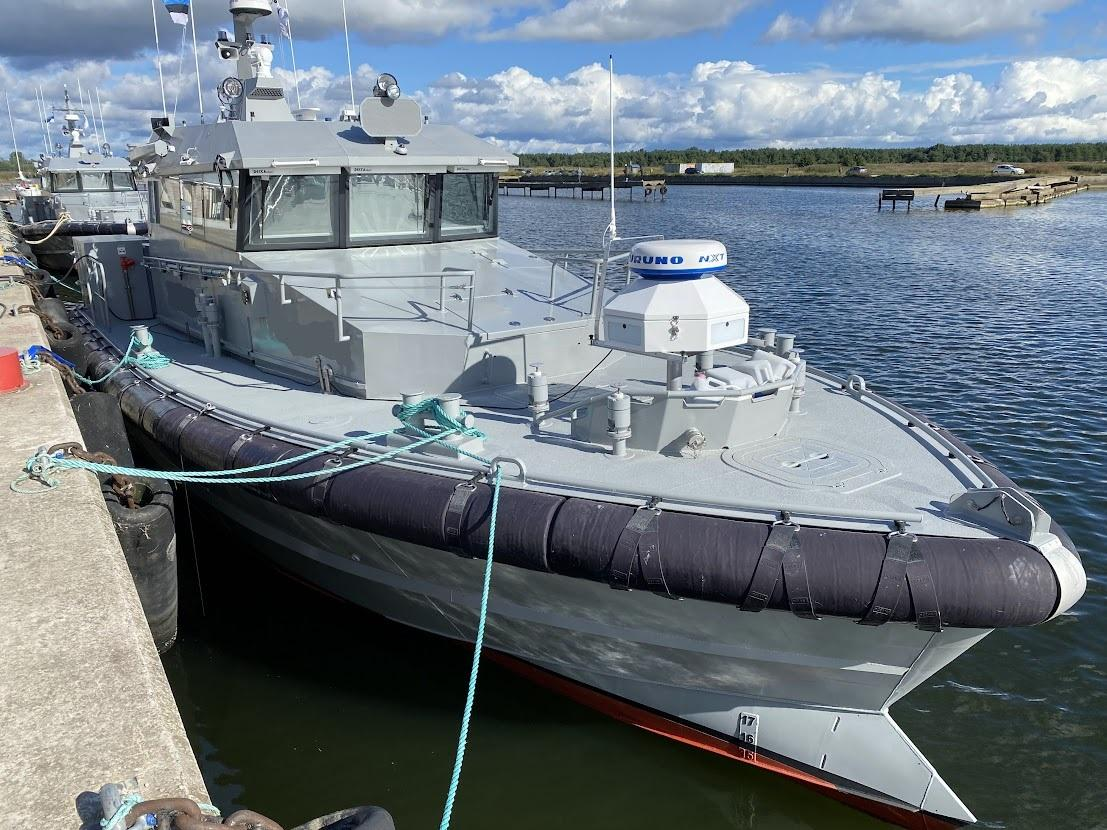
\includegraphics[width=6.10174in,height=4.56944in]{media/image11.jpg}

Joonis 3.4.2. Juhttorni asetus patrulllaeval \cite{ref35}
